\subsection{Introduction}
The goal of this first part is to implement a minimal working simulation of a QAM communication.
In order to achieve that, the up- and downsampling blocks, the RRC filtering blocks and the baseband equivalent model of the channel, as represented in figure~\ref{fig:chain} must be implemented.
\begin{figure}[htbp]
\centering
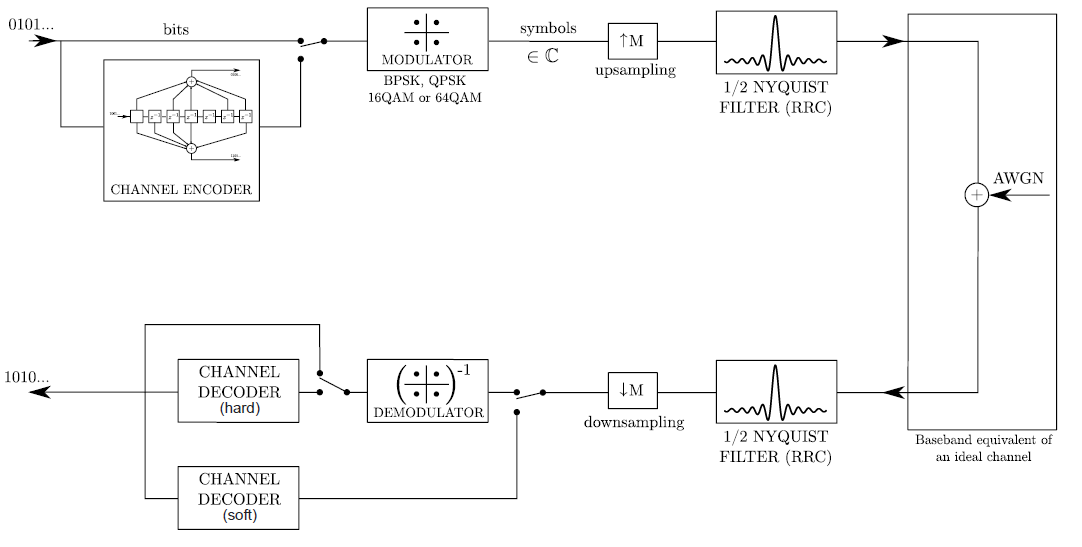
\includegraphics[width=\textwidth]{block.png}
\caption{Block diagram of the communication system [source: Assignment introduction].\label{fig:chain}}
\end{figure}
The modulator and demodulator are supplied with the assignment statement.

\subsection{Halfroot Nyquist filtering}
After its modulation, the message is upsampled and filtered with a root raised cosine filter to limit its bandwidth occupation.
The effect on the PSD of the signal is shown in figure~\ref{fig:LPF}.
\begin{figure}[htbp]
\centering
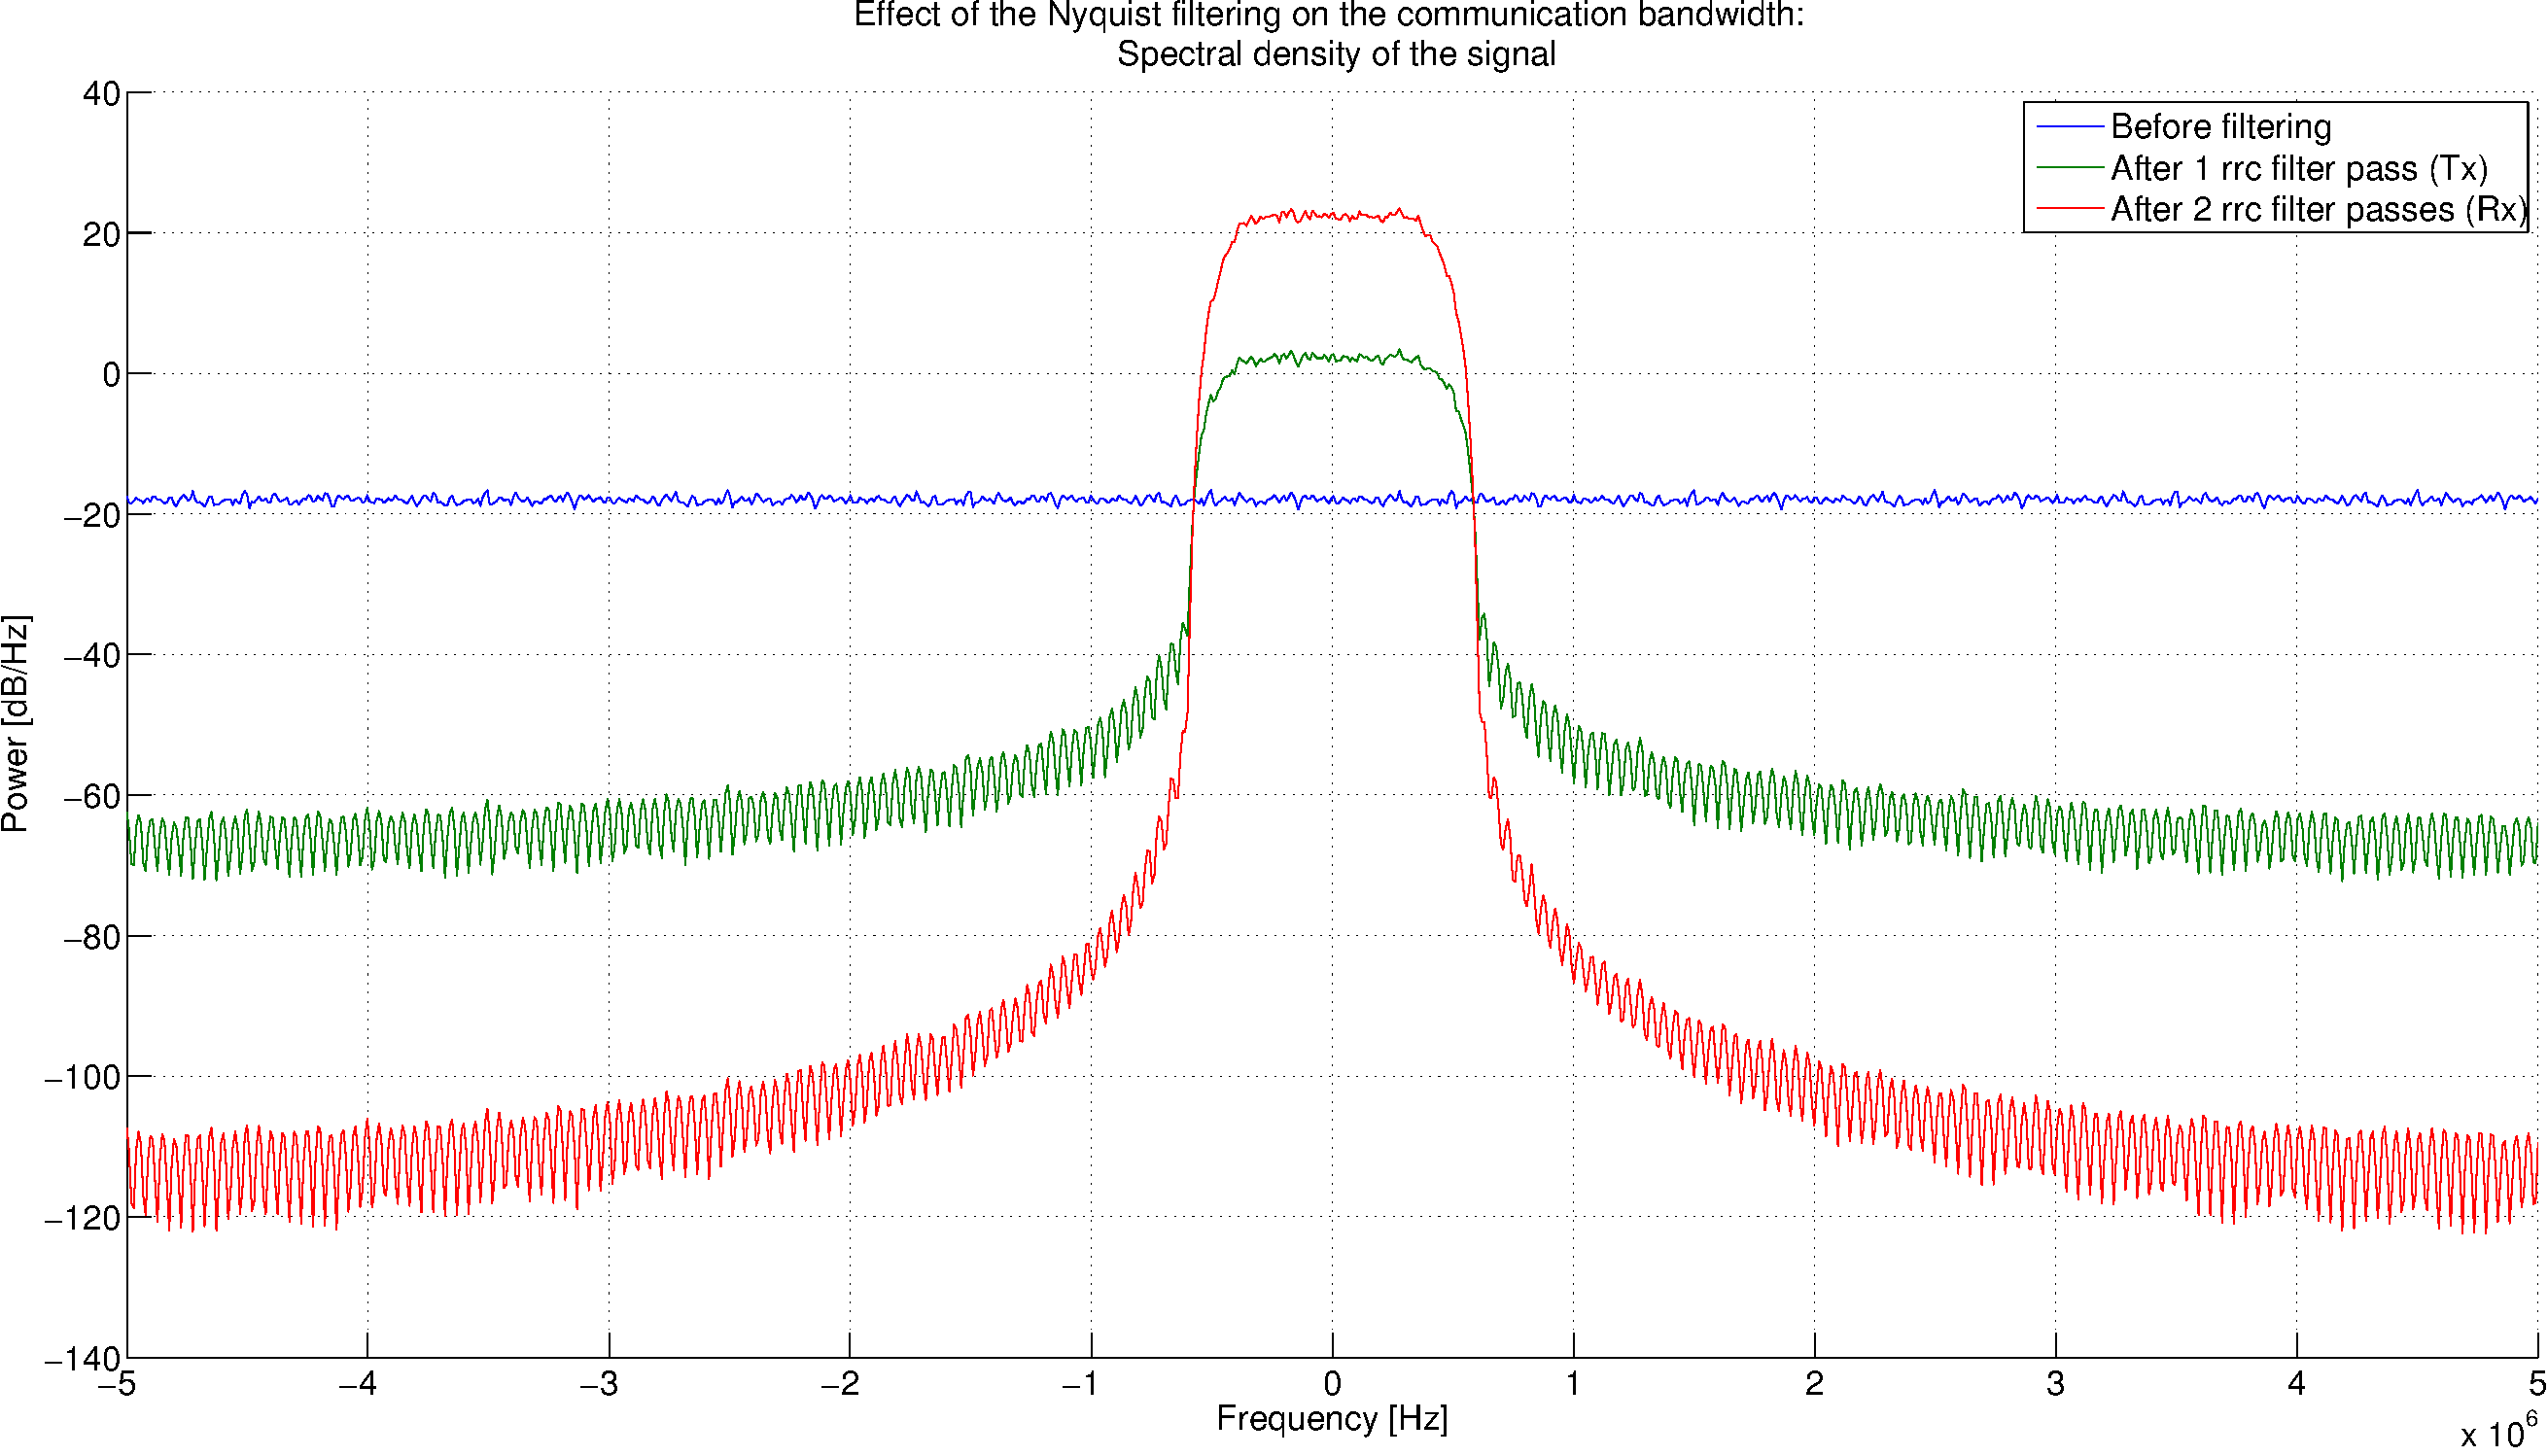
\includegraphics[width=\textwidth]{commBW.pdf}
\caption{Nyquist filtering limits the communication bandwidth. $\beta = 0.3$, $n_{taps} = 20$ $f_m = \SI{1}{\mega\hertz}.$ \label{fig:LPF}}
\end{figure}

In order to maximize the SNR at the output, the low pass filtering is split between the transmitter and the receiver.
The halfroot nyquist filter $g(t)$ is such that the resulting operation $h(t) = g(t)*g(t)$ forms a nyquist filter which does not introduce inter symbol interference, as shown in figure~\ref{fig:noISI}.
\begin{figure}
\centering
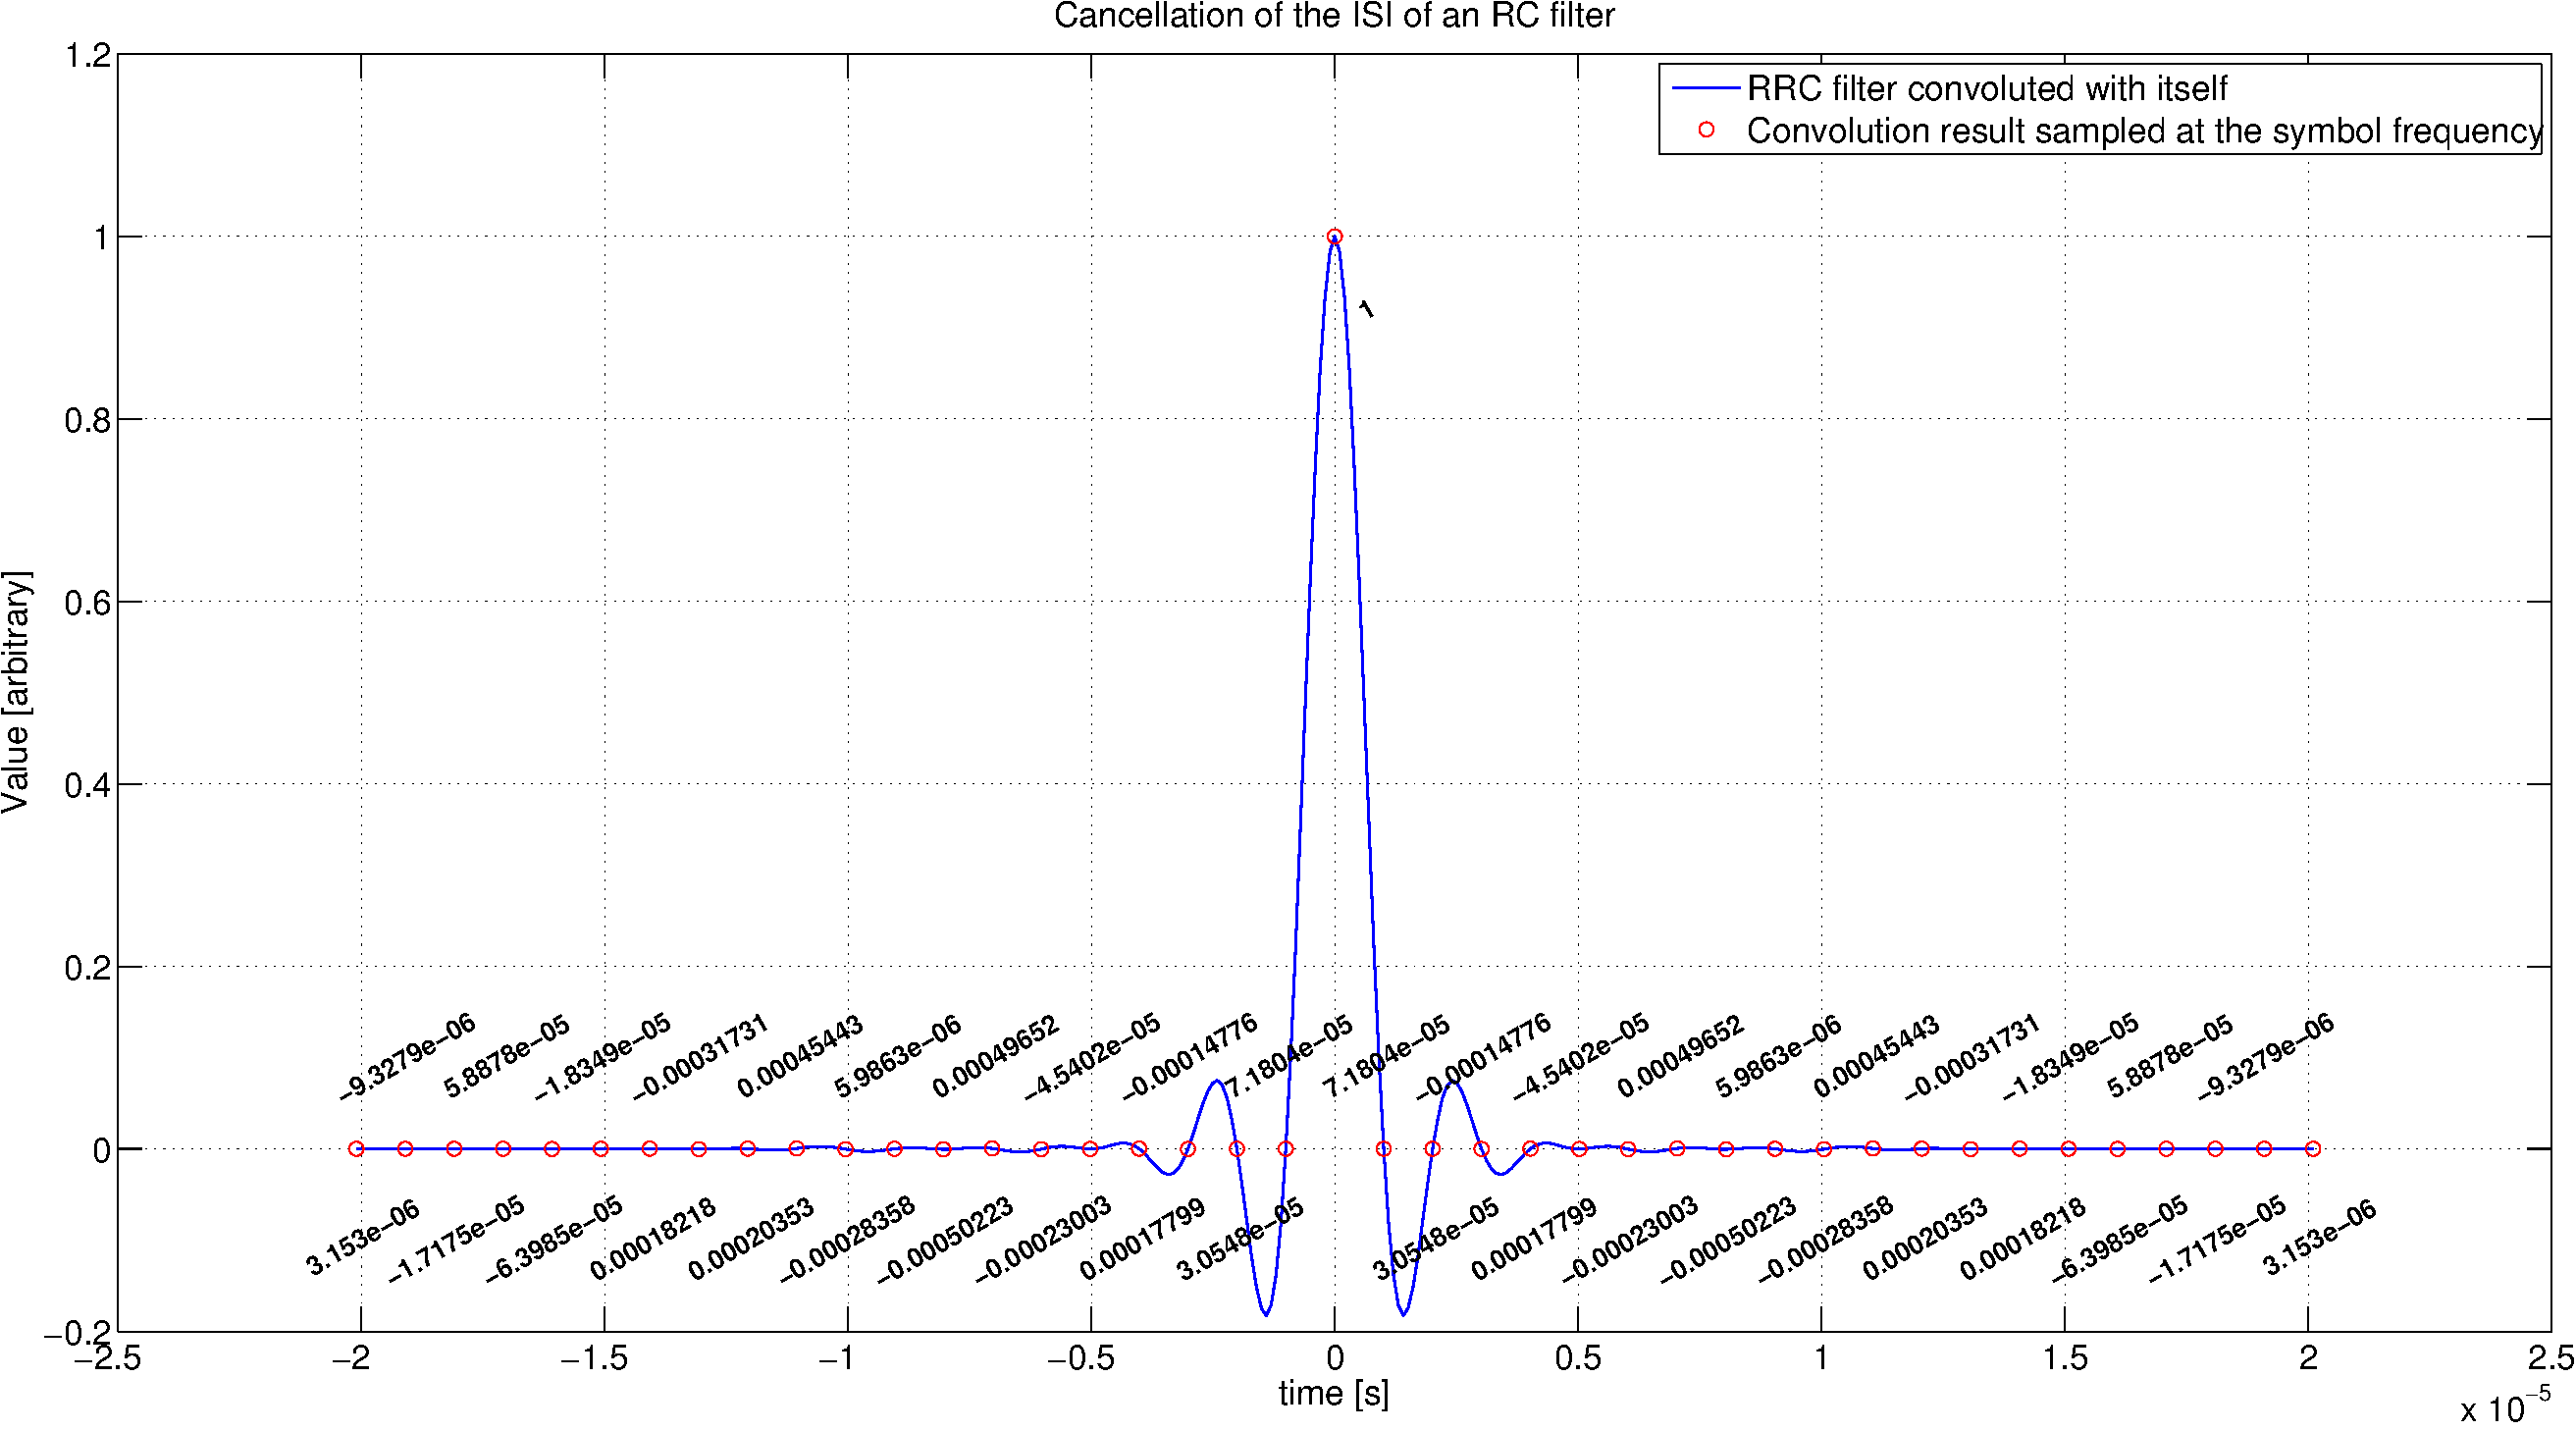
\includegraphics[width = \textwidth]{isi.pdf}
\caption{Cancellation of the inter symbol interference of a raised cosine filter. $\beta = 0.3$, $n_{taps} = 20$ $f_m = \SI{1}{\mega\hertz}.$\label{fig:noISI}}
\end{figure}

\subsection{Impact of the noisy channel}
Theory shows that a channel affected by AWGN can be modelled in the baseband by AWGN of corresponding power.
This allows to easily simulate the BER of the noisy channel.
The results of the simulations are summarized by the BER curves of figure~\ref{fig:BER}.
\begin{figure}[htbp]
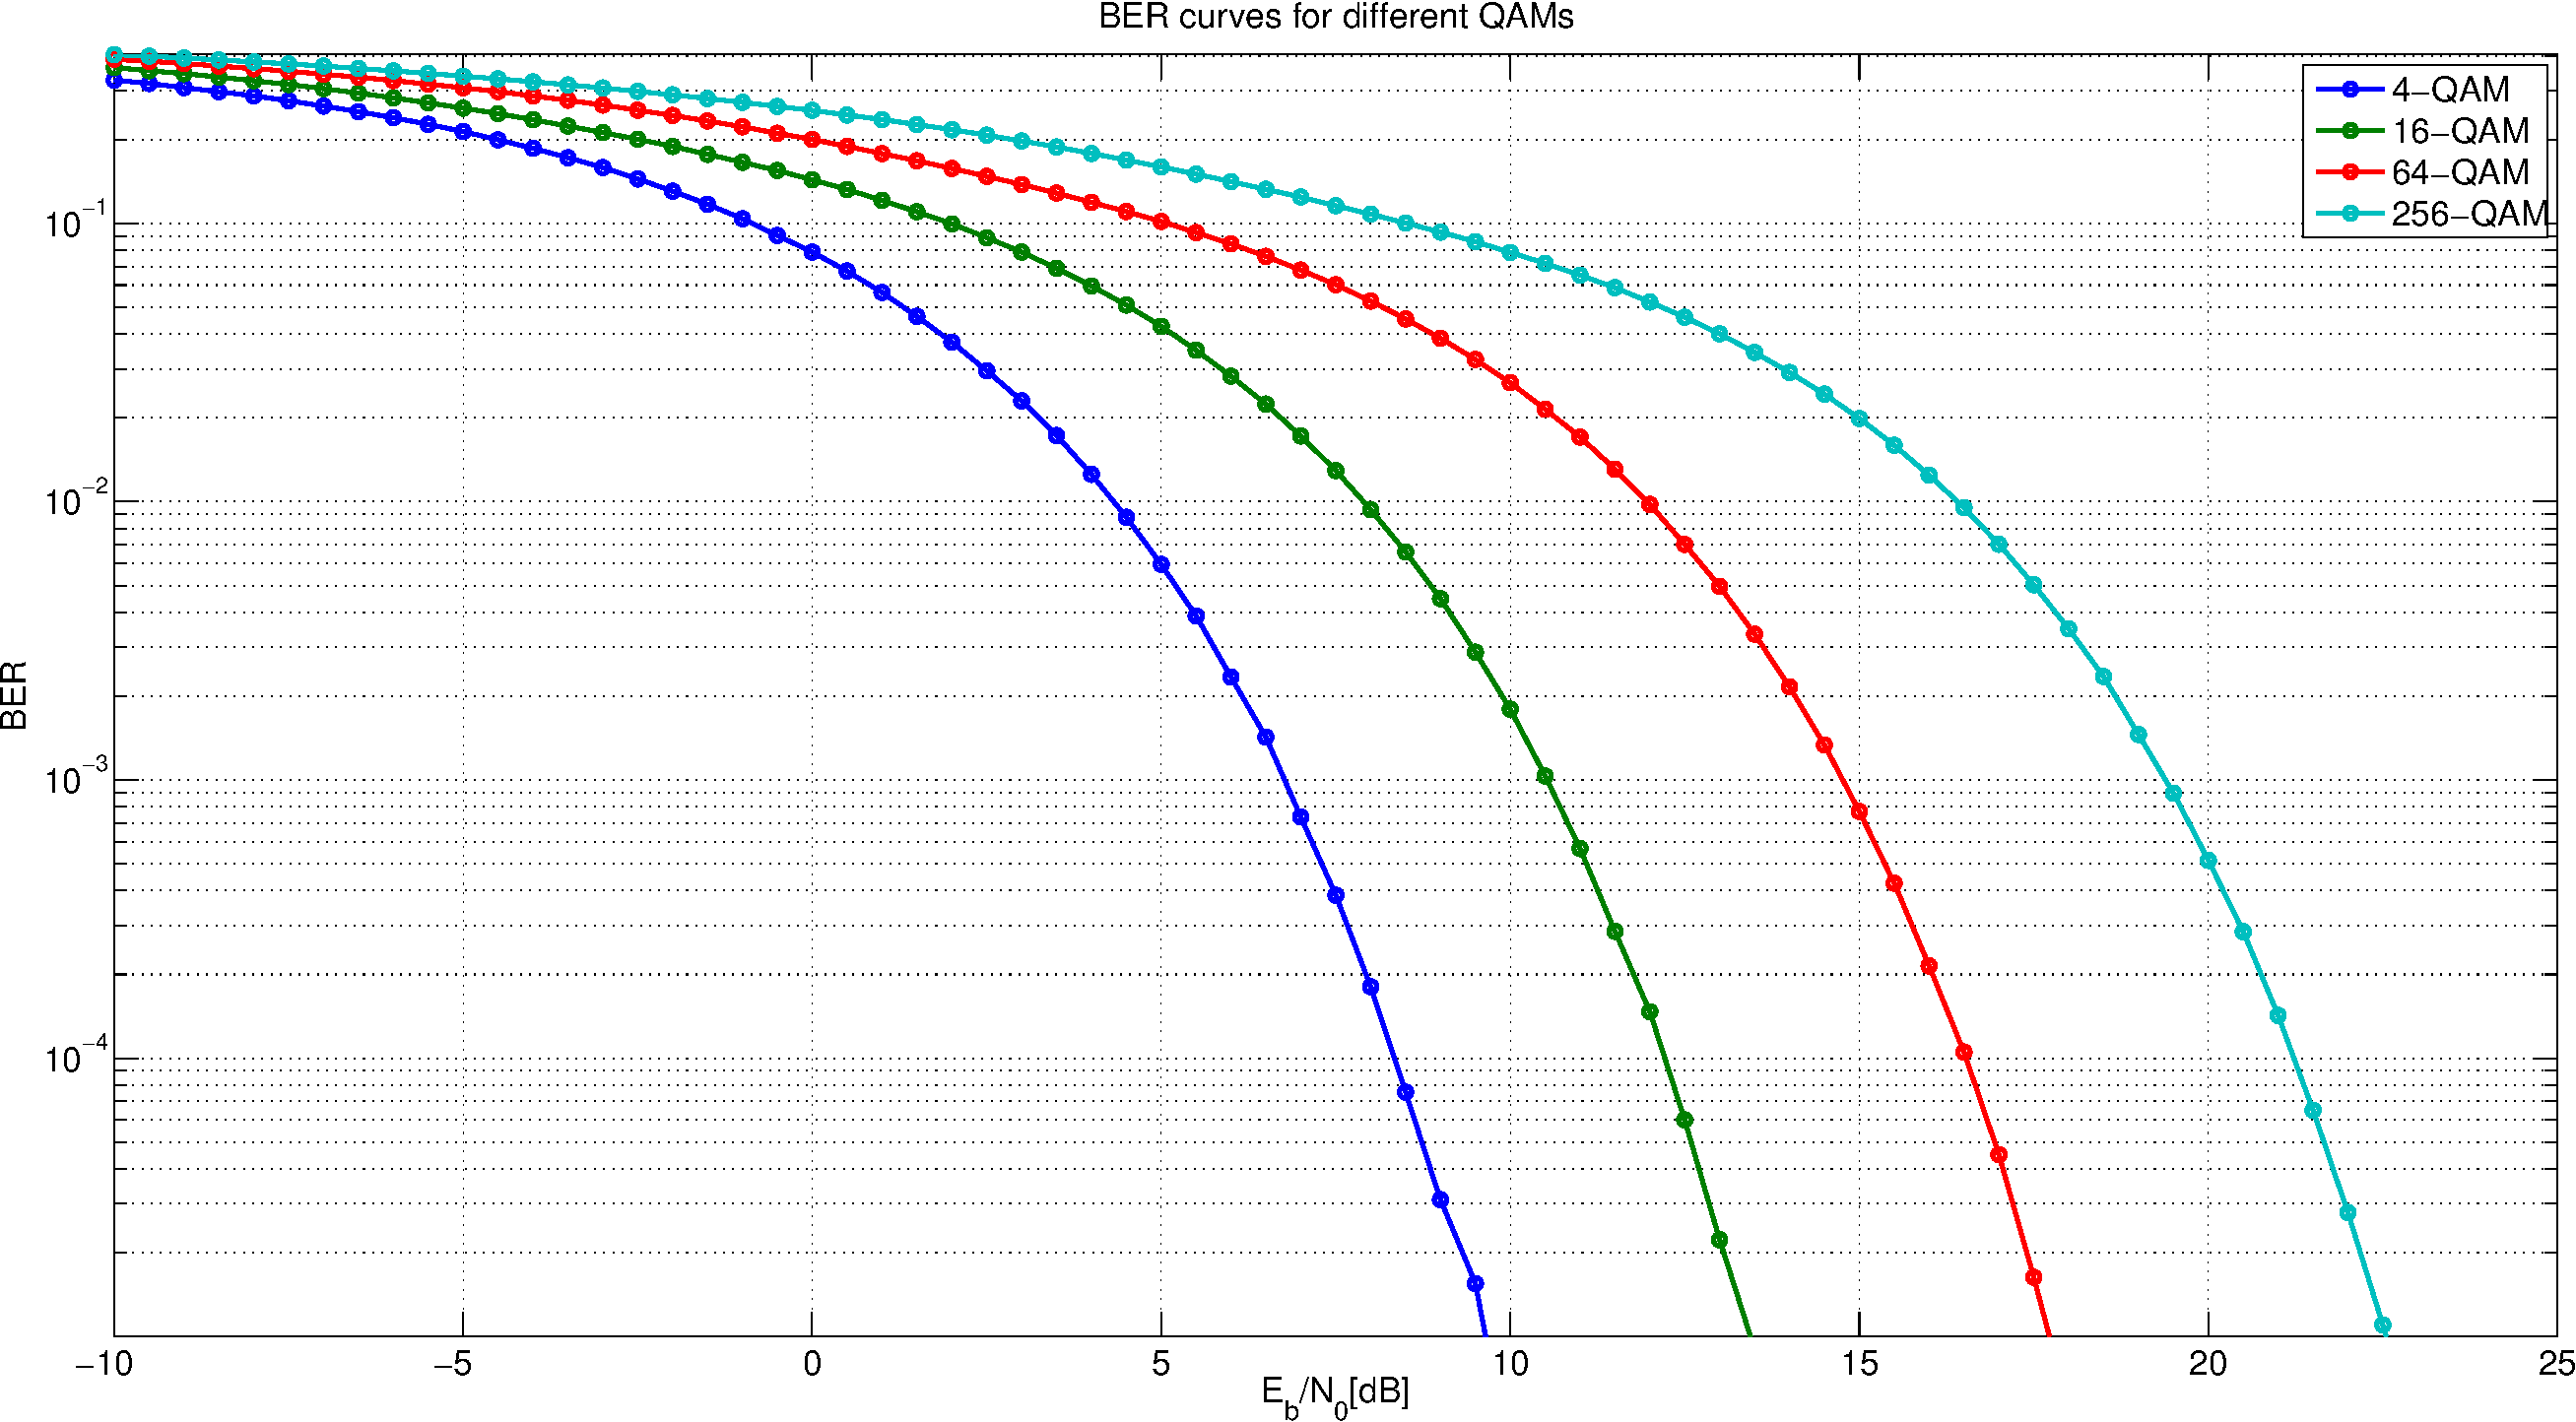
\includegraphics[width=\textwidth]{BER.pdf}
\caption{BER in function of $\frac{E_b}{N_0}$ for different QAM modulations.\label{fig:BER}}
\end{figure}

\subsection{Questions}
\subsubsection{Simulation}
\paragraph{It is proposed to use the baseband equivalent model of the AWGN channel. Would it be
possible to live with a bandpass implementation of the system?}
Simulating in the baseband has the advantage of reducing the sampling frequency needed (at least roughly twice the carrier frequency, which is unrealistic for modern \si{\giga\hertz} links) and allowing to implement and simulate modulation and demodulation techniques regardless of this carrier frequency.
This is why baseband equivalent is always preferred in modelling wireless communication channels.
\paragraph{How do you choose the sample rate in Matlab?}
To be able to observe the effects of Nyquist filtering, the sampling rate must be at least twice as high as the symbol frequency. To be able to simulate sample time shift, even higher sampling rates should be used.
\paragraph{How do you make sure you simulate the desired $\frac{E_b}{N_0}$ ratio?}
Rather than adding a predetermined amount of noise to the signal, we first estimate its power in the useful frequency band, and then choose the noise power in order to obtain the required $\frac{E_b}{N_0}$ ratio.
\paragraph{How do you choose the number of transmitted data packets and their length?}
In order to reliably observe a BER of $10^{-n}$, common practice is to send $10^{n+1}$ bits of data. We can send those in one simulation because the system is time invariant and the noise is ergodic.
\subsubsection{Communication System}
\paragraph{Determine the supported (uncoded) bit rate as a function of the physical bandwidth.} Obviously, R = log2(M)/T with R = bit rate, M = number of symbols and T = symbol duration. With Nyquist filtering: T = 1/FM which is the bandwidth occupied by the signal (see figure~\ref{fig:LPF}).
\paragraph{Explain the trade-off communication capacity/reliability achieved by varying the constellation size.}
As the constellation size increases for a given SNR, the distance between the "edges" of the constellations spots that are spread out by the noise decreases, which means overlaps and thus errors get more and more frequent.
\paragraph{Why do we choose the halfroot Nyquist filter to shape the complex symbols?}
Filtering is required at the transmitter in order to limit the bandwidth used by the transmission. However, ideally, filtering is also needed at the receiver in order to maximize the SNR, since the external noise can affect all frequencies. This is why we choose to split the filtering operation between the transmitter and the receiver. Finally, ISI cancellation is required in order to be able to demodulate the signal properly. This is achieved by splitting a raised cosine filter between the transmitter and the receiver.
\paragraph{How do we implement the optimal demodulator? Give the optimisation criterion.}

\paragraph{How do we implement the optimal detector? Give the optimisation criterion.}
